\begin{longtable}{|r l p{5cm}|p{3cm}|}
\hline
\multicolumn{3}{|c|}{Fonte} & Requisito\tabularnewline
\hline
 &  & Capitolato & \hyperlink{R-3V1}{R-3V1}

\hyperlink{R-3V2}{R-3V2}

\hyperlink{R-3V3}{R-3V3}

\hyperlink{R-3V3.1}{R-3V3.1}

\hyperlink{R-3V3.2}{R-3V3.2}

\hyperlink{R-3V4}{R-3V4}

\hyperlink{R-3V3.3}{R-3V3.3}

\hyperlink{R-3V5}{R-3V5}

\hyperlink{R-3V6}{R-3V6}

\hyperlink{R-3V6.1}{R-3V6.1}

\hyperlink{R-3V6.2}{R-3V6.2}

\hyperlink{R-3F7.1}{R-3F7.1}

\hyperlink{R-3F7.5.1}{R-3F7.5.1}

\hyperlink{R-3F7.2}{R-3F7.2}

\hyperlink{R-3F7.3}{R-3F7.3}

\hyperlink{R-2F7.5.2}{R-2F7.5.2}

\hyperlink{R-3F7.4}{R-3F7.4}

\hyperlink{R-3F7.5}{R-3F7.5}

\hyperlink{R-3F7}{R-3F7}

\hyperlink{R-3F7.7}{R-3F7.7}

\hyperlink{R-3F8}{R-3F8}

\hyperlink{R-3F9}{R-3F9}

\hyperlink{R-3V11}{R-3V11}

\hyperlink{R-3V3.4}{R-3V3.4}

\hyperlink{R-2F7.8}{R-2F7.8}

\hyperlink{R-2F7.9}{R-2F7.9}

\hyperlink{R-2F7.10}{R-2F7.10}

\hyperlink{R-2F7.10.1}{R-2F7.10.1}

\hyperlink{R-2F7.10.2}{R-2F7.10.2}

\hyperlink{R-2F7.10.3}{R-2F7.10.3}

\hyperlink{R-3F7.5.5}{R-3F7.5.5}

\hyperlink{R-3F7.5.1.2}{R-3F7.5.1.2}\tabularnewline
\hline
 &  & Proponente & \hyperlink{R-3F7.5.3}{R-3F7.5.3}

\hyperlink{R-2F7.5.4}{R-2F7.5.4}

\hyperlink{R-2F7.6}{R-2F7.6}\tabularnewline
\hline
 &  & Committente & \tabularnewline
\hline
 &  & Interno & \hyperlink{R-3V11}{R-3V11}

\hyperlink{R-3F10.1}{R-3F10.1}

\hyperlink{R-3F19.1}{R-3F19.1}

\hyperlink{R-3Q26}{R-3Q26}

\hyperlink{R-3Q27}{R-3Q27}

\hyperlink{R-3Q28}{R-3Q28}

\hyperlink{R-2Q29}{R-2Q29}\tabularnewline
\hline
 & \hyperlink{UC1}{UC1} & \hyperlink{UC1}{Autenticazione} & \tabularnewline
\hline
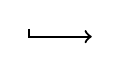
\begin{tikzpicture}
\draw [->, thick] (0.2,0.2) -- (0.2,0.1) -- (1,0.1);
\end{tikzpicture} & \hyperlink{UC1.1}{UC1.1} & \hyperlink{UC1.1}{Inserimento username} & \tabularnewline
\hline
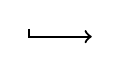
\begin{tikzpicture}
\draw [->, thick] (0.2,0.2) -- (0.2,0.1) -- (1,0.1);
\end{tikzpicture} & \hyperlink{UC1.2}{UC1.2} & \hyperlink{UC1.2}{Inserimento password} & \tabularnewline
\hline
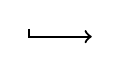
\begin{tikzpicture}
\draw [->, thick] (0.2,0.2) -- (0.2,0.1) -- (1,0.1);
\end{tikzpicture} & \hyperlink{UC1.3}{UC1.3} & \hyperlink{UC1.3}{Errore username non presente} & \tabularnewline
\hline
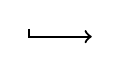
\begin{tikzpicture}
\draw [->, thick] (0.2,0.2) -- (0.2,0.1) -- (1,0.1);
\end{tikzpicture} & \hyperlink{UC1.4}{UC1.4} & \hyperlink{UC1.4}{Errore password errata} & \tabularnewline
\hline
 & \hyperlink{UC2}{UC2} & \hyperlink{UC2}{Registrazione} & \hyperlink{R-3F10}{R-3F10}\tabularnewline
\hline
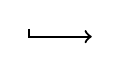
\begin{tikzpicture}
\draw [->, thick] (0.2,0.2) -- (0.2,0.1) -- (1,0.1);
\end{tikzpicture} & \hyperlink{UC2.1}{UC2.1} & \hyperlink{UC2.1}{Inserimento nome completo} & \hyperlink{R-3F10.2}{R-3F10.2}

\hyperlink{R-3F10.2.2}{R-3F10.2.2}\tabularnewline
\hline
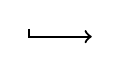
\begin{tikzpicture}
\draw [->, thick] (0.2,0.2) -- (0.2,0.1) -- (1,0.1);
\end{tikzpicture} & \hyperlink{UC2.2}{UC2.2} & \hyperlink{UC2.2}{Inserimento username} & \hyperlink{R-3F10.2}{R-3F10.2}\tabularnewline
\hline
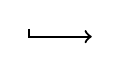
\begin{tikzpicture}
\draw [->, thick] (0.2,0.2) -- (0.2,0.1) -- (1,0.1);
\end{tikzpicture} & \hyperlink{UC2.3}{UC2.3} & \hyperlink{UC2.3}{Inserimento password} & \hyperlink{R-3F10.2}{R-3F10.2}\tabularnewline
\hline
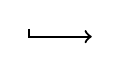
\begin{tikzpicture}
\draw [->, thick] (0.2,0.2) -- (0.2,0.1) -- (1,0.1);
\end{tikzpicture} & \hyperlink{UC2.4}{UC2.4} & \hyperlink{UC2.4}{Errore nome completo troppo corto} & \hyperlink{R-3F10.2.1}{R-3F10.2.1}\tabularnewline
\hline
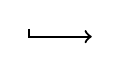
\begin{tikzpicture}
\draw [->, thick] (0.2,0.2) -- (0.2,0.1) -- (1,0.1);
\end{tikzpicture} & \hyperlink{UC2.5}{UC2.5} & \hyperlink{UC2.5}{Errore username troppo corto} & \hyperlink{R-3F10.2.1}{R-3F10.2.1}\tabularnewline
\hline
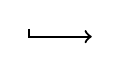
\begin{tikzpicture}
\draw [->, thick] (0.2,0.2) -- (0.2,0.1) -- (1,0.1);
\end{tikzpicture} & \hyperlink{UC2.6}{UC2.6} & \hyperlink{UC2.6}{Errore password troppo corta} & \hyperlink{R-3F10.4}{R-3F10.4}

\hyperlink{R-3F10.2.1}{R-3F10.2.1}\tabularnewline
\hline
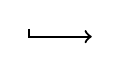
\begin{tikzpicture}
\draw [->, thick] (0.2,0.2) -- (0.2,0.1) -- (1,0.1);
\end{tikzpicture} & \hyperlink{UC2.7}{UC2.7} & \hyperlink{UC2.7}{Errore username già utilizzato} & \hyperlink{R-3F10.3}{R-3F10.3}

\hyperlink{R-3F10.5}{R-3F10.5}

\hyperlink{R-3F10.2.1}{R-3F10.2.1}\tabularnewline
\hline
 & \hyperlink{UC3}{UC3} & \hyperlink{UC3}{Gestione profilo} & \hyperlink{R-3F14}{R-3F14}

\hyperlink{R-3F14.1}{R-3F14.1}

\hyperlink{R-3F14.2}{R-3F14.2}

\hyperlink{R-3F14.1.1}{R-3F14.1.1}

\hyperlink{R-3F14.2.1}{R-3F14.2.1}

\hyperlink{R-3F14.3}{R-3F14.3}

\hyperlink{R-3F14.3.1}{R-3F14.3.1}

\hyperlink{R-3F14.3.2}{R-3F14.3.2}

\hyperlink{R-3F14.2.1.1}{R-3F14.2.1.1}

\hyperlink{R-3F14.2.2}{R-3F14.2.2}

\hyperlink{R-3F14.2.2.1}{R-3F14.2.2.1}

\hyperlink{R-3F14.3.3}{R-3F14.3.3}

\hyperlink{R-3F14.1.2}{R-3F14.1.2}

\hyperlink{R-3F14.3.4}{R-3F14.3.4}\tabularnewline
\hline
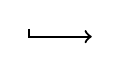
\begin{tikzpicture}
\draw [->, thick] (0.2,0.2) -- (0.2,0.1) -- (1,0.1);
\end{tikzpicture} & \hyperlink{UC3.1}{UC3.1} & \hyperlink{UC3.1}{Modifica nome completo} & \hyperlink{R-3F14.3}{R-3F14.3}

\hyperlink{R-3F14.3.1}{R-3F14.3.1}

\hyperlink{R-3F14.3.3}{R-3F14.3.3}\tabularnewline
\hline
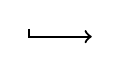
\begin{tikzpicture}
\draw [->, thick] (0.2,0.2) -- (0.2,0.1) -- (1,0.1);
\end{tikzpicture} & \hyperlink{UC3.2}{UC3.2} & \hyperlink{UC3.2}{Modifica username} & \hyperlink{R-3F14.1}{R-3F14.1}

\hyperlink{R-3F14.1.1}{R-3F14.1.1}

\hyperlink{R-3F14.3}{R-3F14.3}

\hyperlink{R-3F14.3.2}{R-3F14.3.2}

\hyperlink{R-3F14.3.4}{R-3F14.3.4}\tabularnewline
\hline
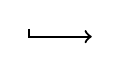
\begin{tikzpicture}
\draw [->, thick] (0.2,0.2) -- (0.2,0.1) -- (1,0.1);
\end{tikzpicture} & \hyperlink{UC3.3}{UC3.3} & \hyperlink{UC3.3}{Modifica password} & \hyperlink{R-3F14.2}{R-3F14.2}

\hyperlink{R-3F14.2.1}{R-3F14.2.1}

\hyperlink{R-3F14.2.2}{R-3F14.2.2}

\hyperlink{R-3F14.2.2.1}{R-3F14.2.2.1}\tabularnewline
\hline
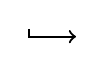
\begin{tikzpicture}
\draw [->, thick] (0.4,0.2) -- (0.4,0.1) -- (1,0.1);
\end{tikzpicture} & \hyperlink{UC3.3.1}{UC3.3.1} & \hyperlink{UC3.3.1}{Inserimento vecchia password} & \hyperlink{R-3F14.2.1}{R-3F14.2.1}\tabularnewline
\hline
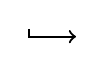
\begin{tikzpicture}
\draw [->, thick] (0.4,0.2) -- (0.4,0.1) -- (1,0.1);
\end{tikzpicture} & \hyperlink{UC3.3.2}{UC3.3.2} & \hyperlink{UC3.3.2}{Errore password non corrispondenti} & \hyperlink{R-3F14.2.1.1}{R-3F14.2.1.1}\tabularnewline
\hline
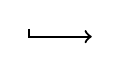
\begin{tikzpicture}
\draw [->, thick] (0.2,0.2) -- (0.2,0.1) -- (1,0.1);
\end{tikzpicture} & \hyperlink{UC3.4}{UC3.4} & \hyperlink{UC3.4}{Errore username troppo corto} & \hyperlink{R-3F14.1.1}{R-3F14.1.1}

\hyperlink{R-3F14.3.4}{R-3F14.3.4}\tabularnewline
\hline
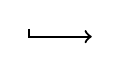
\begin{tikzpicture}
\draw [->, thick] (0.2,0.2) -- (0.2,0.1) -- (1,0.1);
\end{tikzpicture} & \hyperlink{UC3.5}{UC3.5} & \hyperlink{UC3.5}{Errore nome completo troppo corto} & \hyperlink{R-3F14.3.3}{R-3F14.3.3}\tabularnewline
\hline
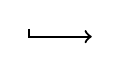
\begin{tikzpicture}
\draw [->, thick] (0.2,0.2) -- (0.2,0.1) -- (1,0.1);
\end{tikzpicture} & \hyperlink{UC3.6}{UC3.6} & \hyperlink{UC3.6}{Errore username già utilizzato} & \hyperlink{R-3F14.1.1}{R-3F14.1.1}

\hyperlink{R-3F14.1.2}{R-3F14.1.2}\tabularnewline
\hline
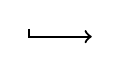
\begin{tikzpicture}
\draw [->, thick] (0.2,0.2) -- (0.2,0.1) -- (1,0.1);
\end{tikzpicture} & \hyperlink{UC3.7}{UC3.7} & \hyperlink{UC3.7}{Errore password troppo corta} & \hyperlink{R-3F14.2.1.1}{R-3F14.2.1.1}

\hyperlink{R-3F14.2.2.1}{R-3F14.2.2.1}\tabularnewline
\hline
 & \hyperlink{UC4}{UC4} & \hyperlink{UC4}{Logout} & \hyperlink{R-3F18}{R-3F18}\tabularnewline
\hline
 & \hyperlink{UC5}{UC5} & \hyperlink{UC5}{Gestione domande} & \hyperlink{R-3F7.2}{R-3F7.2}

\hyperlink{R-3F7.11}{R-3F7.11}

\hyperlink{R-3F7.11.1}{R-3F7.11.1}

\hyperlink{R-3F7.11.2}{R-3F7.11.2}

\hyperlink{R-3F7.11.3}{R-3F7.11.3}

\hyperlink{R-3F7.11.1.1}{R-3F7.11.1.1}

\hyperlink{R-3F7.11.1.2}{R-3F7.11.1.2}

\hyperlink{R-3F7.11.1.1.1}{R-3F7.11.1.1.1}

\hyperlink{R-3F7.11.1.2.1}{R-3F7.11.1.2.1}\tabularnewline
\hline
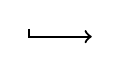
\begin{tikzpicture}
\draw [->, thick] (0.2,0.2) -- (0.2,0.1) -- (1,0.1);
\end{tikzpicture} & \hyperlink{UC5.1}{UC5.1} & \hyperlink{UC5.1}{Inserimento domanda} & \hyperlink{R-2F7.5.2}{R-2F7.5.2}

\hyperlink{R-3F7.5.3}{R-3F7.5.3}

\hyperlink{R-3F7.11.1}{R-3F7.11.1}

\hyperlink{R-3F7.11.1.1}{R-3F7.11.1.1}

\hyperlink{R-3F7.11.1.2.2}{R-3F7.11.1.2.2}

\hyperlink{R-3F7.11.1.2.3}{R-3F7.11.1.2.3}

\hyperlink{R-1F7.11.1.2.4}{R-1F7.11.1.2.4}

\hyperlink{R-1F7.11.1.2.5}{R-1F7.11.1.2.5}

\hyperlink{R-1F7.11.1.2.6}{R-1F7.11.1.2.6}

\hyperlink{R-2F7.11.1.2.7}{R-2F7.11.1.2.7}

\hyperlink{R-3F7.5.5}{R-3F7.5.5}\tabularnewline
\hline
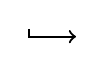
\begin{tikzpicture}
\draw [->, thick] (0.4,0.2) -- (0.4,0.1) -- (1,0.1);
\end{tikzpicture} & \hyperlink{UC5.1.1}{UC5.1.1} & \hyperlink{UC5.1.1}{Selezione argomenti nuova domanda} & \hyperlink{R-3F7.11.1.1}{R-3F7.11.1.1}

\hyperlink{R-3F7.11.1.1.1}{R-3F7.11.1.1.1}\tabularnewline
\hline
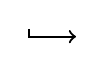
\begin{tikzpicture}
\draw [->, thick] (0.4,0.2) -- (0.4,0.1) -- (1,0.1);
\end{tikzpicture} & \hyperlink{UC5.1.2}{UC5.1.2} & \hyperlink{UC5.1.2}{Scrittura domanda in QML della nuova domanda} & \hyperlink{R-3F7.5.1}{R-3F7.5.1}

\hyperlink{R-3F7.5}{R-3F7.5}

\hyperlink{R-3F7.11.1.2}{R-3F7.11.1.2}

\hyperlink{R-3F7.11.1.2.1}{R-3F7.11.1.2.1}

\hyperlink{R-2F7.5.1.1}{R-2F7.5.1.1}

\hyperlink{R-3F7.5.1.2}{R-3F7.5.1.2}

\hyperlink{R-2F7.5.1.3}{R-2F7.5.1.3}

\hyperlink{R-2F7.5.1.4}{R-2F7.5.1.4}

\hyperlink{R-2F7.5.1.5}{R-2F7.5.1.5}

\hyperlink{R-3F7.5.1.6}{R-3F7.5.1.6}

\hyperlink{R-2F7.5.1.7}{R-2F7.5.1.7}

\hyperlink{R-2F7.5.1.8}{R-2F7.5.1.8}\tabularnewline
\hline
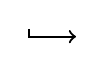
\begin{tikzpicture}
\draw [->, thick] (0.4,0.2) -- (0.4,0.1) -- (1,0.1);
\end{tikzpicture} & \hyperlink{UC5.1.3}{UC5.1.3} & \hyperlink{UC5.1.3}{Scrittura nuova domanda da interfaccia grafica} & \hyperlink{R-2F7.5.4}{R-2F7.5.4}

\hyperlink{R-2F7.5.1.7}{R-2F7.5.1.7}

\hyperlink{R-2F7.5.1.8}{R-2F7.5.1.8}\tabularnewline
\hline
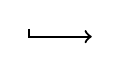
\begin{tikzpicture}
\draw [->, thick] (0.2,0.2) -- (0.2,0.1) -- (1,0.1);
\end{tikzpicture} & \hyperlink{UC5.2}{UC5.2} & \hyperlink{UC5.2}{Modifica domanda} & \hyperlink{R-3F7.11.2}{R-3F7.11.2}\tabularnewline
\hline
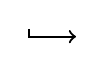
\begin{tikzpicture}
\draw [->, thick] (0.4,0.2) -- (0.4,0.1) -- (1,0.1);
\end{tikzpicture} & \hyperlink{UC5.2.1}{UC5.2.1} & \hyperlink{UC5.2.1}{Selezione argomenti modifica domanda} & \tabularnewline
\hline
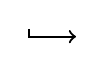
\begin{tikzpicture}
\draw [->, thick] (0.4,0.2) -- (0.4,0.1) -- (1,0.1);
\end{tikzpicture} & \hyperlink{UC5.2.2}{UC5.2.2} & \hyperlink{UC5.2.2}{Scrittura domanda in QML della domanda da modificare} & \tabularnewline
\hline
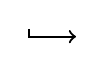
\begin{tikzpicture}
\draw [->, thick] (0.4,0.2) -- (0.4,0.1) -- (1,0.1);
\end{tikzpicture} & \hyperlink{UC5.2.3}{UC5.2.3} & \hyperlink{UC5.2.3}{Modifica domanda da interfaccia grafica} & \tabularnewline
\hline
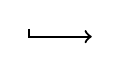
\begin{tikzpicture}
\draw [->, thick] (0.2,0.2) -- (0.2,0.1) -- (1,0.1);
\end{tikzpicture} & \hyperlink{UC5.3}{UC5.3} & \hyperlink{UC5.3}{Elimina domanda} & \hyperlink{R-3F7.11.3}{R-3F7.11.3}\tabularnewline
\hline
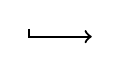
\begin{tikzpicture}
\draw [->, thick] (0.2,0.2) -- (0.2,0.1) -- (1,0.1);
\end{tikzpicture} & \hyperlink{UC5.4}{UC5.4} & \hyperlink{UC5.4}{Errore QML non valido} & \hyperlink{R-3F7.11.1.2.1}{R-3F7.11.1.2.1}\tabularnewline
\hline
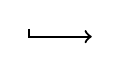
\begin{tikzpicture}
\draw [->, thick] (0.2,0.2) -- (0.2,0.1) -- (1,0.1);
\end{tikzpicture} & \hyperlink{UC5.5}{UC5.5} & \hyperlink{UC5.5}{Errore argomento mancante} & \hyperlink{R-3F7.11.1.1.1}{R-3F7.11.1.1.1}\tabularnewline
\hline
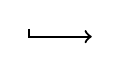
\begin{tikzpicture}
\draw [->, thick] (0.2,0.2) -- (0.2,0.1) -- (1,0.1);
\end{tikzpicture} & \hyperlink{UC5.6}{UC5.6} & \hyperlink{UC5.6}{Inserimento domanda di tipo vero/falso} & \hyperlink{R-3F7.11.1.2.2}{R-3F7.11.1.2.2}

\hyperlink{R-3F7.5.5}{R-3F7.5.5}\tabularnewline
\hline
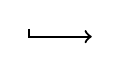
\begin{tikzpicture}
\draw [->, thick] (0.2,0.2) -- (0.2,0.1) -- (1,0.1);
\end{tikzpicture} & \hyperlink{UC5.7}{UC5.7} & \hyperlink{UC5.7}{Inserimento domanda a scelta multipla} & \hyperlink{R-2F7.5.2}{R-2F7.5.2}

\hyperlink{R-3F7.11.1.2.3}{R-3F7.11.1.2.3}\tabularnewline
\hline
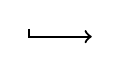
\begin{tikzpicture}
\draw [->, thick] (0.2,0.2) -- (0.2,0.1) -- (1,0.1);
\end{tikzpicture} & \hyperlink{UC5.8}{UC5.8} & \hyperlink{UC5.8}{Inserimento domanda a risposta multipla} & \hyperlink{R-1F7.11.1.2.4}{R-1F7.11.1.2.4}

\hyperlink{R-3F7.5.5}{R-3F7.5.5}\tabularnewline
\hline
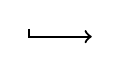
\begin{tikzpicture}
\draw [->, thick] (0.2,0.2) -- (0.2,0.1) -- (1,0.1);
\end{tikzpicture} & \hyperlink{UC5.9}{UC5.9} & \hyperlink{UC5.9}{Inserimento domanda di tipo testo con parole omesse} & \hyperlink{R-2F7.5.2}{R-2F7.5.2}

\hyperlink{R-1F7.11.1.2.5}{R-1F7.11.1.2.5}\tabularnewline
\hline
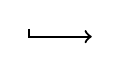
\begin{tikzpicture}
\draw [->, thick] (0.2,0.2) -- (0.2,0.1) -- (1,0.1);
\end{tikzpicture} & \hyperlink{UC5.10}{UC5.10} & \hyperlink{UC5.10}{Inserimento domanda con l'associazione di parole} & \hyperlink{R-2F7.5.2}{R-2F7.5.2}

\hyperlink{R-1F7.11.1.2.6}{R-1F7.11.1.2.6}\tabularnewline
\hline
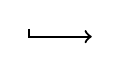
\begin{tikzpicture}
\draw [->, thick] (0.2,0.2) -- (0.2,0.1) -- (1,0.1);
\end{tikzpicture} & \hyperlink{UC5.11}{UC5.11} & \hyperlink{UC5.11}{Inserimento domanda a risposta aperta} & \hyperlink{R-2F7.5.2}{R-2F7.5.2}

\hyperlink{R-2F7.11.1.2.7}{R-2F7.11.1.2.7}\tabularnewline
\hline
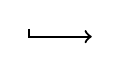
\begin{tikzpicture}
\draw [->, thick] (0.2,0.2) -- (0.2,0.1) -- (1,0.1);
\end{tikzpicture} & \hyperlink{UC5.12}{UC5.12} & \hyperlink{UC5.12}{Visualizza domanda} & \hyperlink{R-3F7.2}{R-3F7.2}

\hyperlink{R-3F30}{R-3F30}\tabularnewline
\hline
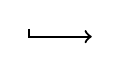
\begin{tikzpicture}
\draw [->, thick] (0.2,0.2) -- (0.2,0.1) -- (1,0.1);
\end{tikzpicture} & \hyperlink{UC5.13}{UC5.13} & \hyperlink{UC5.13}{Errore eliminazione domanda utilizzata} & \tabularnewline
\hline
 & \hyperlink{UC6}{UC6} & \hyperlink{UC6}{Gestione questionari} & \hyperlink{R-3F7.2}{R-3F7.2}

\hyperlink{R-3F7.3}{R-3F7.3}

\hyperlink{R-3F7}{R-3F7}

\hyperlink{R-3F7.7}{R-3F7.7}

\hyperlink{R-3F7.11}{R-3F7.11}

\hyperlink{R-3F7.12}{R-3F7.12}

\hyperlink{R-3F7.12.2}{R-3F7.12.2}

\hyperlink{R-3F7.12.3}{R-3F7.12.3}

\hyperlink{R-3F7.13}{R-3F7.13}

\hyperlink{R-3F7.12.4}{R-3F7.12.4}

\hyperlink{R-3F7.7.1}{R-3F7.7.1}\tabularnewline
\hline
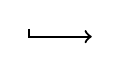
\begin{tikzpicture}
\draw [->, thick] (0.2,0.2) -- (0.2,0.1) -- (1,0.1);
\end{tikzpicture} & \hyperlink{UC6.1}{UC6.1} & \hyperlink{UC6.1}{Inserisci questionario} & \hyperlink{R-3F7.7}{R-3F7.7}

\hyperlink{R-3F7.7.1}{R-3F7.7.1}\tabularnewline
\hline
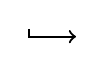
\begin{tikzpicture}
\draw [->, thick] (0.4,0.2) -- (0.4,0.1) -- (1,0.1);
\end{tikzpicture} & \hyperlink{UC6.1.1}{UC6.1.1} & \hyperlink{UC6.1.1}{Aggiungi domanda in un nuovo questionario } & \hyperlink{R-3F7.11}{R-3F7.11}

\hyperlink{R-3F7.11.1.2}{R-3F7.11.1.2}

\hyperlink{R-3F7.11.1.1.1}{R-3F7.11.1.1.1}

\hyperlink{R-3F7.11.1.2.1}{R-3F7.11.1.2.1}\tabularnewline
\hline
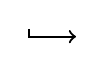
\begin{tikzpicture}
\draw [->, thick] (0.4,0.2) -- (0.4,0.1) -- (1,0.1);
\end{tikzpicture} & \hyperlink{UC6.1.2}{UC6.1.2} & \hyperlink{UC6.1.2}{Elimina domanda da un nuovo questionario} & \hyperlink{R-3F7.11}{R-3F7.11}\tabularnewline
\hline
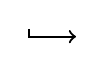
\begin{tikzpicture}
\draw [->, thick] (0.4,0.2) -- (0.4,0.1) -- (1,0.1);
\end{tikzpicture} & \hyperlink{UC6.1.3}{UC6.1.3} & \hyperlink{UC6.1.3}{Seleziona argomenti del nuovo questionario} & \tabularnewline
\hline
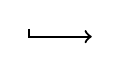
\begin{tikzpicture}
\draw [->, thick] (0.2,0.2) -- (0.2,0.1) -- (1,0.1);
\end{tikzpicture} & \hyperlink{UC6.2}{UC6.2} & \hyperlink{UC6.2}{Modifica questionario} & \hyperlink{R-3F7.12}{R-3F7.12}

\hyperlink{R-3F7.12.4}{R-3F7.12.4}\tabularnewline
\hline
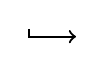
\begin{tikzpicture}
\draw [->, thick] (0.4,0.2) -- (0.4,0.1) -- (1,0.1);
\end{tikzpicture} & \hyperlink{UC6.2.1}{UC6.2.1} & \hyperlink{UC6.2.1}{Aggiungi domanda in un questionario} & \hyperlink{R-3F7.12.2}{R-3F7.12.2}\tabularnewline
\hline
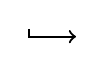
\begin{tikzpicture}
\draw [->, thick] (0.4,0.2) -- (0.4,0.1) -- (1,0.1);
\end{tikzpicture} & \hyperlink{UC6.2.2}{UC6.2.2} & \hyperlink{UC6.2.2}{Elimina domanda da un questionario da  modificare} & \hyperlink{R-3F7.12.3}{R-3F7.12.3}\tabularnewline
\hline
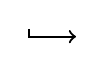
\begin{tikzpicture}
\draw [->, thick] (0.4,0.2) -- (0.4,0.1) -- (1,0.1);
\end{tikzpicture} & \hyperlink{UC6.2.3}{UC6.2.3} & \hyperlink{UC6.2.3}{Selezione argomenti modifica questionario} & \hyperlink{R-3F7.12.4}{R-3F7.12.4}\tabularnewline
\hline
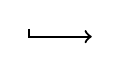
\begin{tikzpicture}
\draw [->, thick] (0.2,0.2) -- (0.2,0.1) -- (1,0.1);
\end{tikzpicture} & \hyperlink{UC6.3}{UC6.3} & \hyperlink{UC6.3}{Elimina questionario} & \hyperlink{R-3F7.13}{R-3F7.13}\tabularnewline
\hline
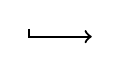
\begin{tikzpicture}
\draw [->, thick] (0.2,0.2) -- (0.2,0.1) -- (1,0.1);
\end{tikzpicture} & \hyperlink{UC6.4}{UC6.4} & \hyperlink{UC6.4}{Errore questionario vuoto} & \hyperlink{R-3F7.7.1}{R-3F7.7.1}\tabularnewline
\hline
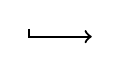
\begin{tikzpicture}
\draw [->, thick] (0.2,0.2) -- (0.2,0.1) -- (1,0.1);
\end{tikzpicture} & \hyperlink{UC6.5}{UC6.5} & \hyperlink{UC6.5}{Visualizza questionario} & \hyperlink{R-3F31}{R-3F31}\tabularnewline
\hline
 & \hyperlink{UC7}{UC7} & \hyperlink{UC7}{Gestione classi} & \hyperlink{R-2F13.1.1}{R-2F13.1.1}

\hyperlink{R-2F13}{R-2F13}

\hyperlink{R-2F13.1}{R-2F13.1}

\hyperlink{R-2F13.2}{R-2F13.2}

\hyperlink{R-2F13.3}{R-2F13.3}

\hyperlink{R-2F13.1.2}{R-2F13.1.2}

\hyperlink{R-2F13.1.3}{R-2F13.1.3}

\hyperlink{R-2F13.3.1}{R-2F13.3.1}

\hyperlink{R-2F13.3.2}{R-2F13.3.2}

\hyperlink{R-2F13.3.3}{R-2F13.3.3}

\hyperlink{R-2F13.1.1.1}{R-2F13.1.1.1}\tabularnewline
\hline
\begin{tikzpicture}
\draw [->, thick] (0.2,0.2) -- (0.2,0.1) -- (1,0.1);
\end{tikzpicture} & \hyperlink{UC7.1}{UC7.1} & \hyperlink{UC7.1}{Inserisci classe} & \hyperlink{R-2F7.6}{R-2F7.6}

\hyperlink{R-2F13.1.1}{R-2F13.1.1}

\hyperlink{R-2F13.1}{R-2F13.1}

\hyperlink{R-2F13.1.2}{R-2F13.1.2}

\hyperlink{R-2F13.1.3}{R-2F13.1.3}

\hyperlink{R-2F13.1.1.1}{R-2F13.1.1.1}\tabularnewline
\hline
\begin{tikzpicture}
\draw [->, thick] (0.4,0.2) -- (0.4,0.1) -- (1,0.1);
\end{tikzpicture} & \hyperlink{UC7.1.1}{UC7.1.1} & \hyperlink{UC7.1.1}{Inserisci nome classe} & \hyperlink{R-2F13.1.1}{R-2F13.1.1}

\hyperlink{R-2F13.3.1}{R-2F13.3.1}

\hyperlink{R-2F13.1.1.1}{R-2F13.1.1.1}\tabularnewline
\hline
\begin{tikzpicture}
\draw [->, thick] (0.4,0.2) -- (0.4,0.1) -- (1,0.1);
\end{tikzpicture} & \hyperlink{UC7.1.2}{UC7.1.2} & \hyperlink{UC7.1.2}{Inserisci argomenti classe} & \hyperlink{R-2F13.1.2}{R-2F13.1.2}

\hyperlink{R-2F13.3.2}{R-2F13.3.2}\tabularnewline
\hline
\begin{tikzpicture}
\draw [->, thick] (0.4,0.2) -- (0.4,0.1) -- (1,0.1);
\end{tikzpicture} & \hyperlink{UC7.1.3}{UC7.1.3} & \hyperlink{UC7.1.3}{Inserisci password classe} & \hyperlink{R-2F13.1.3}{R-2F13.1.3}

\hyperlink{R-2F13.3.3}{R-2F13.3.3}\tabularnewline
\hline
\begin{tikzpicture}
\draw [->, thick] (0.2,0.2) -- (0.2,0.1) -- (1,0.1);
\end{tikzpicture} & \hyperlink{UC7.2}{UC7.2} & \hyperlink{UC7.2}{Modifica classe} & \hyperlink{R-2F13.3}{R-2F13.3}

\hyperlink{R-2F13.3.1}{R-2F13.3.1}

\hyperlink{R-2F13.3.2}{R-2F13.3.2}

\hyperlink{R-2F13.3.3}{R-2F13.3.3}\tabularnewline
\hline
\begin{tikzpicture}
\draw [->, thick] (0.2,0.2) -- (0.2,0.1) -- (1,0.1);
\end{tikzpicture} & \hyperlink{UC7.3}{UC7.3} & \hyperlink{UC7.3}{Elimina classe} & \hyperlink{R-2F13.2}{R-2F13.2}\tabularnewline
\hline
\begin{tikzpicture}
\draw [->, thick] (0.2,0.2) -- (0.2,0.1) -- (1,0.1);
\end{tikzpicture} & \hyperlink{UC7.4}{UC7.4} & \hyperlink{UC7.4}{Errore nome classe già presente} & \hyperlink{R-2F13.1.1.1}{R-2F13.1.1.1}\tabularnewline
\hline
 & \hyperlink{UC8}{UC8} & \hyperlink{UC8}{Gestione argomenti} & \hyperlink{R-3F23}{R-3F23}

\hyperlink{R-3F23.1}{R-3F23.1}

\hyperlink{R-3F23.2}{R-3F23.2}

\hyperlink{R-3F23.3}{R-3F23.3}

\hyperlink{R-3F23.4}{R-3F23.4}

\hyperlink{R-3F23.1.1}{R-3F23.1.1}

\hyperlink{R-3F23.2.1}{R-3F23.2.1}

\hyperlink{R-3F23.2.2}{R-3F23.2.2}\tabularnewline
\hline
\begin{tikzpicture}
\draw [->, thick] (0.2,0.2) -- (0.2,0.1) -- (1,0.1);
\end{tikzpicture} & \hyperlink{UC8.1}{UC8.1} & \hyperlink{UC8.1}{Esplorazione argomenti} & \hyperlink{R-3F23.4}{R-3F23.4}

\hyperlink{R-3F23.2.1}{R-3F23.2.1}\tabularnewline
\hline
\begin{tikzpicture}
\draw [->, thick] (0.2,0.2) -- (0.2,0.1) -- (1,0.1);
\end{tikzpicture} & \hyperlink{UC8.2}{UC8.2} & \hyperlink{UC8.2}{Crea argomento} & \hyperlink{R-3F23.1}{R-3F23.1}

\hyperlink{R-3F23.1.1}{R-3F23.1.1}\tabularnewline
\hline
\begin{tikzpicture}
\draw [->, thick] (0.2,0.2) -- (0.2,0.1) -- (1,0.1);
\end{tikzpicture} & \hyperlink{UC8.3}{UC8.3} & \hyperlink{UC8.3}{Argomento già presente nel sistema} & \hyperlink{R-3F23.1.1}{R-3F23.1.1}\tabularnewline
\hline
\begin{tikzpicture}
\draw [->, thick] (0.2,0.2) -- (0.2,0.1) -- (1,0.1);
\end{tikzpicture} & \hyperlink{UC8.4}{UC8.4} & \hyperlink{UC8.4}{Modifica argomento} & \hyperlink{R-3F23.3}{R-3F23.3}\tabularnewline
\hline
\begin{tikzpicture}
\draw [->, thick] (0.2,0.2) -- (0.2,0.1) -- (1,0.1);
\end{tikzpicture} & \hyperlink{UC8.5}{UC8.5} & \hyperlink{UC8.5}{Eliminazione argomento} & \hyperlink{R-3F23.2}{R-3F23.2}

\hyperlink{R-3F23.2.1}{R-3F23.2.1}

\hyperlink{R-3F23.2.2}{R-3F23.2.2}\tabularnewline
\hline
\begin{tikzpicture}
\draw [->, thick] (0.2,0.2) -- (0.2,0.1) -- (1,0.1);
\end{tikzpicture} & \hyperlink{UC8.6}{UC8.6} & \hyperlink{UC8.6}{Errore l'argomento ha domande o questionari} & \hyperlink{R-3F23.2.2}{R-3F23.2.2}\tabularnewline
\hline
 & \hyperlink{UC9}{UC9} & \hyperlink{UC9}{Visualizza statistiche} & \hyperlink{R-2F24.3.1}{R-2F24.3.1}

\hyperlink{R-2F24}{R-2F24}

\hyperlink{R-2F24.1}{R-2F24.1}

\hyperlink{R-2F24.2}{R-2F24.2}

\hyperlink{R-2F24.3}{R-2F24.3}

\hyperlink{R-2F24.1.1}{R-2F24.1.1}

\hyperlink{R-2F24.2.1}{R-2F24.2.1}

\hyperlink{R-2F24.3.2}{R-2F24.3.2}

\hyperlink{R-2F24.3.3}{R-2F24.3.3}

\hyperlink{R-2F24.3.4}{R-2F24.3.4}

\hyperlink{R-2F24.3.4.1}{R-2F24.3.4.1}

\hyperlink{R-2F24.3.5}{R-2F24.3.5}

\hyperlink{R-2F24.3.5.1}{R-2F24.3.5.1}\tabularnewline
\hline
 & \hyperlink{UC10}{UC10} & \hyperlink{UC10}{Visualizza statistiche domanda} & \hyperlink{R-2F24.1}{R-2F24.1}

\hyperlink{R-2F24.1.1}{R-2F24.1.1}\tabularnewline
\hline
 & \hyperlink{UC11}{UC11} & \hyperlink{UC11}{Visualizza statistiche questionario} & \hyperlink{R-2F24.2}{R-2F24.2}

\hyperlink{R-2F24.2.1}{R-2F24.2.1}\tabularnewline
\hline
 & \hyperlink{UC12}{UC12} & \hyperlink{UC12}{Visualizza statistiche classe} & \hyperlink{R-2F24.3.1}{R-2F24.3.1}

\hyperlink{R-2F24.3}{R-2F24.3}

\hyperlink{R-2F24.3.2}{R-2F24.3.2}

\hyperlink{R-2F24.3.3}{R-2F24.3.3}

\hyperlink{R-2F24.3.4}{R-2F24.3.4}

\hyperlink{R-2F24.3.4.1}{R-2F24.3.4.1}

\hyperlink{R-2F24.3.5}{R-2F24.3.5}

\hyperlink{R-2F24.3.5.1}{R-2F24.3.5.1}\tabularnewline
\hline
\begin{tikzpicture}
\draw [->, thick] (0.2,0.2) -- (0.2,0.1) -- (1,0.1);
\end{tikzpicture} & \hyperlink{UC12.1}{UC12.1} & \hyperlink{UC12.1}{Visualizza risultati domande della classe} & \hyperlink{R-2F24.3.5}{R-2F24.3.5}

\hyperlink{R-2F24.3.5.1}{R-2F24.3.5.1}\tabularnewline
\hline
\begin{tikzpicture}
\draw [->, thick] (0.2,0.2) -- (0.2,0.1) -- (1,0.1);
\end{tikzpicture} & \hyperlink{UC12.2}{UC12.2} & \hyperlink{UC12.2}{Visualizza risultati questionari della classe} & \hyperlink{R-2F24.3.1}{R-2F24.3.1}\tabularnewline
\hline
\begin{tikzpicture}
\draw [->, thick] (0.2,0.2) -- (0.2,0.1) -- (1,0.1);
\end{tikzpicture} & \hyperlink{UC12.3}{UC12.3} & \hyperlink{UC12.3}{Visualizza sommario statistiche classe} & \hyperlink{R-2F24.3.3}{R-2F24.3.3}\tabularnewline
\hline
\begin{tikzpicture}
\draw [->, thick] (0.2,0.2) -- (0.2,0.1) -- (1,0.1);
\end{tikzpicture} & \hyperlink{UC12.4}{UC12.4} & \hyperlink{UC12.4}{Visualizza statistiche studente della classe} & \hyperlink{R-2F24.3.4}{R-2F24.3.4}

\hyperlink{R-2F24.3.4.1}{R-2F24.3.4.1}\tabularnewline
\hline
\begin{tikzpicture}
\draw [->, thick] (0.4,0.2) -- (0.4,0.1) -- (1,0.1);
\end{tikzpicture} & \hyperlink{UC12.4.1}{UC12.4.1} & \hyperlink{UC12.4.1}{Visualizza risultati questionari dello studente} & \hyperlink{R-2F24.3.4.1}{R-2F24.3.4.1}\tabularnewline
\hline
 & \hyperlink{UC13}{UC13} & \hyperlink{UC13}{Esegui questionario} & \hyperlink{R-3F7.4}{R-3F7.4}

\hyperlink{R-3F17}{R-3F17}

\hyperlink{R-3F17.1}{R-3F17.1}

\hyperlink{R-3F17.2}{R-3F17.2}

\hyperlink{R-3F17.3}{R-3F17.3}

\hyperlink{R-3F17.4}{R-3F17.4}

\hyperlink{R-3F17.2.1}{R-3F17.2.1}\tabularnewline
\hline
\begin{tikzpicture}
\draw [->, thick] (0.2,0.2) -- (0.2,0.1) -- (1,0.1);
\end{tikzpicture} & \hyperlink{UC13.1}{UC13.1} & \hyperlink{UC13.1}{Rispondi domanda} & \hyperlink{R-3F7.2}{R-3F7.2}

\hyperlink{R-3F8}{R-3F8}

\hyperlink{R-3F17.1}{R-3F17.1}

\hyperlink{R-3F17.1.1}{R-3F17.1.1}

\hyperlink{R-3F17.1.2}{R-3F17.1.2}

\hyperlink{R-1F17.1.3}{R-1F17.1.3}

\hyperlink{R-1F17.1.4}{R-1F17.1.4}

\hyperlink{R-1F17.1.5}{R-1F17.1.5}

\hyperlink{R-2F17.1.6}{R-2F17.1.6}\tabularnewline
\hline
\begin{tikzpicture}
\draw [->, thick] (0.2,0.2) -- (0.2,0.1) -- (1,0.1);
\end{tikzpicture} & \hyperlink{UC13.2}{UC13.2} & \hyperlink{UC13.2}{Errore domanda non risposta} & \hyperlink{R-3F17.2.1}{R-3F17.2.1}\tabularnewline
\hline
\begin{tikzpicture}
\draw [->, thick] (0.2,0.2) -- (0.2,0.1) -- (1,0.1);
\end{tikzpicture} & \hyperlink{UC13.3}{UC13.3} & \hyperlink{UC13.3}{Conferma questionario} & \hyperlink{R-3F17.2}{R-3F17.2}

\hyperlink{R-3F17.2.1}{R-3F17.2.1}\tabularnewline
\hline
\begin{tikzpicture}
\draw [->, thick] (0.2,0.2) -- (0.2,0.1) -- (1,0.1);
\end{tikzpicture} & \hyperlink{UC13.4}{UC13.4} & \hyperlink{UC13.4}{Rispondi domanda vero/falso} & \hyperlink{R-3F17.1.1}{R-3F17.1.1}\tabularnewline
\hline
\begin{tikzpicture}
\draw [->, thick] (0.2,0.2) -- (0.2,0.1) -- (1,0.1);
\end{tikzpicture} & \hyperlink{UC13.5}{UC13.5} & \hyperlink{UC13.5}{Rispondi domanda a scelta multipla} & \hyperlink{R-3F17.1.2}{R-3F17.1.2}\tabularnewline
\hline
\begin{tikzpicture}
\draw [->, thick] (0.2,0.2) -- (0.2,0.1) -- (1,0.1);
\end{tikzpicture} & \hyperlink{UC13.6}{UC13.6} & \hyperlink{UC13.6}{Rispondi domanda a risposta multipla} & \hyperlink{R-1F17.1.3}{R-1F17.1.3}\tabularnewline
\hline
\begin{tikzpicture}
\draw [->, thick] (0.2,0.2) -- (0.2,0.1) -- (1,0.1);
\end{tikzpicture} & \hyperlink{UC13.7}{UC13.7} & \hyperlink{UC13.7}{Rispondi domanda di tipo testo con parole omesse} & \hyperlink{R-1F17.1.4}{R-1F17.1.4}\tabularnewline
\hline
\begin{tikzpicture}
\draw [->, thick] (0.2,0.2) -- (0.2,0.1) -- (1,0.1);
\end{tikzpicture} & \hyperlink{UC13.8}{UC13.8} & \hyperlink{UC13.8}{Rispondi domanda con associazione di parole} & \hyperlink{R-1F17.1.5}{R-1F17.1.5}\tabularnewline
\hline
\begin{tikzpicture}
\draw [->, thick] (0.2,0.2) -- (0.2,0.1) -- (1,0.1);
\end{tikzpicture} & \hyperlink{UC13.9}{UC13.9} & \hyperlink{UC13.9}{Rispondi domanda a risposta aperta} & \hyperlink{R-2F17.1.6}{R-2F17.1.6}\tabularnewline
\hline
\begin{tikzpicture}
\draw [->, thick] (0.2,0.2) -- (0.2,0.1) -- (1,0.1);
\end{tikzpicture} & \hyperlink{UC13.10}{UC13.10} & \hyperlink{UC13.10}{Feedback questionario} & \hyperlink{R-2F7.9}{R-2F7.9}\tabularnewline
\hline
\begin{tikzpicture}
\draw [->, thick] (0.2,0.2) -- (0.2,0.1) -- (1,0.1);
\end{tikzpicture} & \hyperlink{UC13.11}{UC13.11} & \hyperlink{UC13.11}{Visualizza valutazione questionario} & \hyperlink{R-3F7.4}{R-3F7.4}\tabularnewline
\hline
 & \hyperlink{UC14}{UC14} & \hyperlink{UC14}{Iscrizione ad una classe} & \hyperlink{R-2F7.6}{R-2F7.6}

\hyperlink{R-2F16}{R-2F16}

\hyperlink{R-2F16.1}{R-2F16.1}

\hyperlink{R-2F16.1.1}{R-2F16.1.1}\tabularnewline
\hline
\begin{tikzpicture}
\draw [->, thick] (0.2,0.2) -- (0.2,0.1) -- (1,0.1);
\end{tikzpicture} & \hyperlink{UC14.1}{UC14.1} & \hyperlink{UC14.1}{Inserisci password classe} & \hyperlink{R-2F16.1}{R-2F16.1}\tabularnewline
\hline
\begin{tikzpicture}
\draw [->, thick] (0.2,0.2) -- (0.2,0.1) -- (1,0.1);
\end{tikzpicture} & \hyperlink{UC14.2}{UC14.2} & \hyperlink{UC14.2}{Errore password classe} & \hyperlink{R-2F16.1.1}{R-2F16.1.1}\tabularnewline
\hline
 & \hyperlink{UC15}{UC15} & \hyperlink{UC15}{Visualizza storico studente} & \hyperlink{R-3F7.4}{R-3F7.4}

\hyperlink{R-2F7.10}{R-2F7.10}

\hyperlink{R-2F7.10.1}{R-2F7.10.1}

\hyperlink{R-2F7.10.2}{R-2F7.10.2}

\hyperlink{R-2F7.10.3}{R-2F7.10.3}

\hyperlink{R-2F25}{R-2F25}

\hyperlink{R-2F25.1}{R-2F25.1}

\hyperlink{R-2F25.2}{R-2F25.2}

\hyperlink{R-2F25.3}{R-2F25.3}

\hyperlink{R-2F25.3.1}{R-2F25.3.1}

\hyperlink{R-2F25.1.1}{R-2F25.1.1}

\hyperlink{R-2F25.1.2}{R-2F25.1.2}

\hyperlink{R-2F25.1.3}{R-2F25.1.3}

\hyperlink{R-2F25.1.4}{R-2F25.1.4}

\hyperlink{R-2F25.1.5}{R-2F25.1.5}

\hyperlink{R-2F25.2.1}{R-2F25.2.1}

\hyperlink{R-2F25.2.2}{R-2F25.2.2}

\hyperlink{R-2F25.3.2}{R-2F25.3.2}

\hyperlink{R-2F25.3.3}{R-2F25.3.3}

\hyperlink{R-2F25.3.4}{R-2F25.3.4}\tabularnewline
\hline
\begin{tikzpicture}
\draw [->, thick] (0.2,0.2) -- (0.2,0.1) -- (1,0.1);
\end{tikzpicture} & \hyperlink{UC15.1}{UC15.1} & \hyperlink{UC15.1}{Visualizza statistiche domande studente} & \hyperlink{R-2F25.2}{R-2F25.2}

\hyperlink{R-2F25.2.1}{R-2F25.2.1}

\hyperlink{R-2F25.2.2}{R-2F25.2.2}\tabularnewline
\hline
\begin{tikzpicture}
\draw [->, thick] (0.2,0.2) -- (0.2,0.1) -- (1,0.1);
\end{tikzpicture} & \hyperlink{UC15.2}{UC15.2} & \hyperlink{UC15.2}{Visualizza statistiche questionari studente} & \hyperlink{R-2F7.10.2}{R-2F7.10.2}

\hyperlink{R-2F25.3}{R-2F25.3}

\hyperlink{R-2F25.3.1}{R-2F25.3.1}

\hyperlink{R-2F25.3.2}{R-2F25.3.2}

\hyperlink{R-2F25.3.3}{R-2F25.3.3}

\hyperlink{R-2F25.3.4}{R-2F25.3.4}\tabularnewline
\hline
\begin{tikzpicture}
\draw [->, thick] (0.2,0.2) -- (0.2,0.1) -- (1,0.1);
\end{tikzpicture} & \hyperlink{UC15.3}{UC15.3} & \hyperlink{UC15.3}{Visualizza sommario statistiche studente} & \hyperlink{R-2F7.10.3}{R-2F7.10.3}

\hyperlink{R-2F25.1}{R-2F25.1}

\hyperlink{R-2F25.1.1}{R-2F25.1.1}

\hyperlink{R-2F25.1.2}{R-2F25.1.2}

\hyperlink{R-2F25.1.3}{R-2F25.1.3}

\hyperlink{R-2F25.1.4}{R-2F25.1.4}

\hyperlink{R-2F25.1.5}{R-2F25.1.5}\tabularnewline
\hline
 & \hyperlink{UC16}{UC16} & \hyperlink{UC16}{Ricerca questionario} & \hyperlink{R-3F7.12.1}{R-3F7.12.1}

\hyperlink{R-3F15}{R-3F15}

\hyperlink{R-3F15.1}{R-3F15.1}

\hyperlink{R-2F15.2}{R-2F15.2}

\hyperlink{R-3F15.3}{R-3F15.3}

\hyperlink{R-3F15.4}{R-3F15.4}

\hyperlink{R-2F15.5}{R-2F15.5}

\hyperlink{R-2F24.2.1}{R-2F24.2.1}

\hyperlink{R-2F24.3.4.1}{R-2F24.3.4.1}

\hyperlink{R-2F25.3.1}{R-2F25.3.1}\tabularnewline
\hline
 & \hyperlink{UC17}{UC17} & \hyperlink{UC17}{Ricerca questionario per titolo} & \hyperlink{R-3F15.1}{R-3F15.1}\tabularnewline
\hline
 & \hyperlink{UC18}{UC18} & \hyperlink{UC18}{Ricerca questionario per classe} & \hyperlink{R-2F15.2}{R-2F15.2}\tabularnewline
\hline
 & \hyperlink{UC19}{UC19} & \hyperlink{UC19}{Ricerca questionario per argomento} & \hyperlink{R-3F15.4}{R-3F15.4}\tabularnewline
\hline
 & \hyperlink{UC20}{UC20} & \hyperlink{UC20}{Ricerca questionario per docente} & \hyperlink{R-3F15.3}{R-3F15.3}\tabularnewline
\hline
 & \hyperlink{UC21}{UC21} & \hyperlink{UC21}{Ricerca questionario per difficoltà} & \hyperlink{R-2F15.5}{R-2F15.5}\tabularnewline
\hline
 & \hyperlink{UC22}{UC22} & \hyperlink{UC22}{Ricerca domanda} & \hyperlink{R-3F20}{R-3F20}

\hyperlink{R-3F20.1}{R-3F20.1}

\hyperlink{R-3F20.2}{R-3F20.2}

\hyperlink{R-2F20.3}{R-2F20.3}

\hyperlink{R-3F20.4}{R-3F20.4}

\hyperlink{R-2F24.1.1}{R-2F24.1.1}

\hyperlink{R-2F24.3.5.1}{R-2F24.3.5.1}\tabularnewline
\hline
 & \hyperlink{UC23}{UC23} & \hyperlink{UC23}{Ricerca domanda per keywords} & \hyperlink{R-3F20.4}{R-3F20.4}\tabularnewline
\hline
 & \hyperlink{UC24}{UC24} & \hyperlink{UC24}{Ricerca domanda per argomento} & \hyperlink{R-3F20.1}{R-3F20.1}\tabularnewline
\hline
 & \hyperlink{UC25}{UC25} & \hyperlink{UC25}{Ricerca domanda per difficoltà} & \hyperlink{R-2F20.3}{R-2F20.3}\tabularnewline
\hline
 & \hyperlink{UC26}{UC26} & \hyperlink{UC26}{Ricerca domanda per docente} & \hyperlink{R-3F20.2}{R-3F20.2}\tabularnewline
\hline
 & \hyperlink{UC27}{UC27} & \hyperlink{UC27}{Ricerca classe} & \hyperlink{R-2F16.2}{R-2F16.2}

\hyperlink{R-2F21}{R-2F21}

\hyperlink{R-2F21.1}{R-2F21.1}

\hyperlink{R-2F21.2}{R-2F21.2}\tabularnewline
\hline
 & \hyperlink{UC28}{UC28} & \hyperlink{UC28}{Ricerca classe per docente} & \hyperlink{R-2F16.2}{R-2F16.2}

\hyperlink{R-2F21.2}{R-2F21.2}\tabularnewline
\hline
 & \hyperlink{UC29}{UC29} & \hyperlink{UC29}{Ricerca classe per argomento} & \hyperlink{R-2F16.2}{R-2F16.2}

\hyperlink{R-2F21.1}{R-2F21.1}\tabularnewline
\hline
 & \hyperlink{UC30}{UC30} & \hyperlink{UC30}{Azioni Amministratore} & \hyperlink{R-3F12}{R-3F12}

\hyperlink{R-3F12.1}{R-3F12.1}

\hyperlink{R-3F12.2}{R-3F12.2}

\hyperlink{R-3F19}{R-3F19}

\hyperlink{R-3F19.2}{R-3F19.2}

\hyperlink{R-3F19.3}{R-3F19.3}\tabularnewline
\hline
\begin{tikzpicture}
\draw [->, thick] (0.2,0.2) -- (0.2,0.1) -- (1,0.1);
\end{tikzpicture} & \hyperlink{UC30.1}{UC30.1} & \hyperlink{UC30.1}{Cambia ruolo} & \hyperlink{R-3F12.1}{R-3F12.1}

\hyperlink{R-3F19.2}{R-3F19.2}\tabularnewline
\hline
\begin{tikzpicture}
\draw [->, thick] (0.2,0.2) -- (0.2,0.1) -- (1,0.1);
\end{tikzpicture} & \hyperlink{UC30.2}{UC30.2} & \hyperlink{UC30.2}{Rimozione utente} & \hyperlink{R-3F12.2}{R-3F12.2}

\hyperlink{R-3F19.3}{R-3F19.3}\tabularnewline
\hline
 & \hyperlink{UC31}{UC31} & \hyperlink{UC31}{Ricerca utente} & \tabularnewline
\hline
 & \hyperlink{UC32}{UC32} & \hyperlink{UC32}{Ricerca utente per nome completo} & \tabularnewline
\hline
 & \hyperlink{UC33}{UC33} & \hyperlink{UC33}{Ricerca utente per username} & \tabularnewline
\hline
 & \hyperlink{UC34}{UC34} & \hyperlink{UC34}{Ricerca utente per ruolo} & \tabularnewline
\hline
 & \hyperlink{UC35}{UC35} & \hyperlink{UC35}{Recupero password} & \hyperlink{R-2F22}{R-2F22}

\hyperlink{R-2F22.1}{R-2F22.1}

\hyperlink{R-2F22.2}{R-2F22.2}\tabularnewline
\hline
\begin{tikzpicture}
\draw [->, thick] (0.2,0.2) -- (0.2,0.1) -- (1,0.1);
\end{tikzpicture} & \hyperlink{UC35.1}{UC35.1} & \hyperlink{UC35.1}{Errore mail per recupero password non presente} & \hyperlink{R-2F22.2}{R-2F22.2}\tabularnewline
\hline
\caption{Tabella fonti/requisiti} \tabularnewline
\end{longtable}
